% Created by tikzDevice version 0.11 on 2018-10-22 23:22:36
% !TEX encoding = UTF-8 Unicode
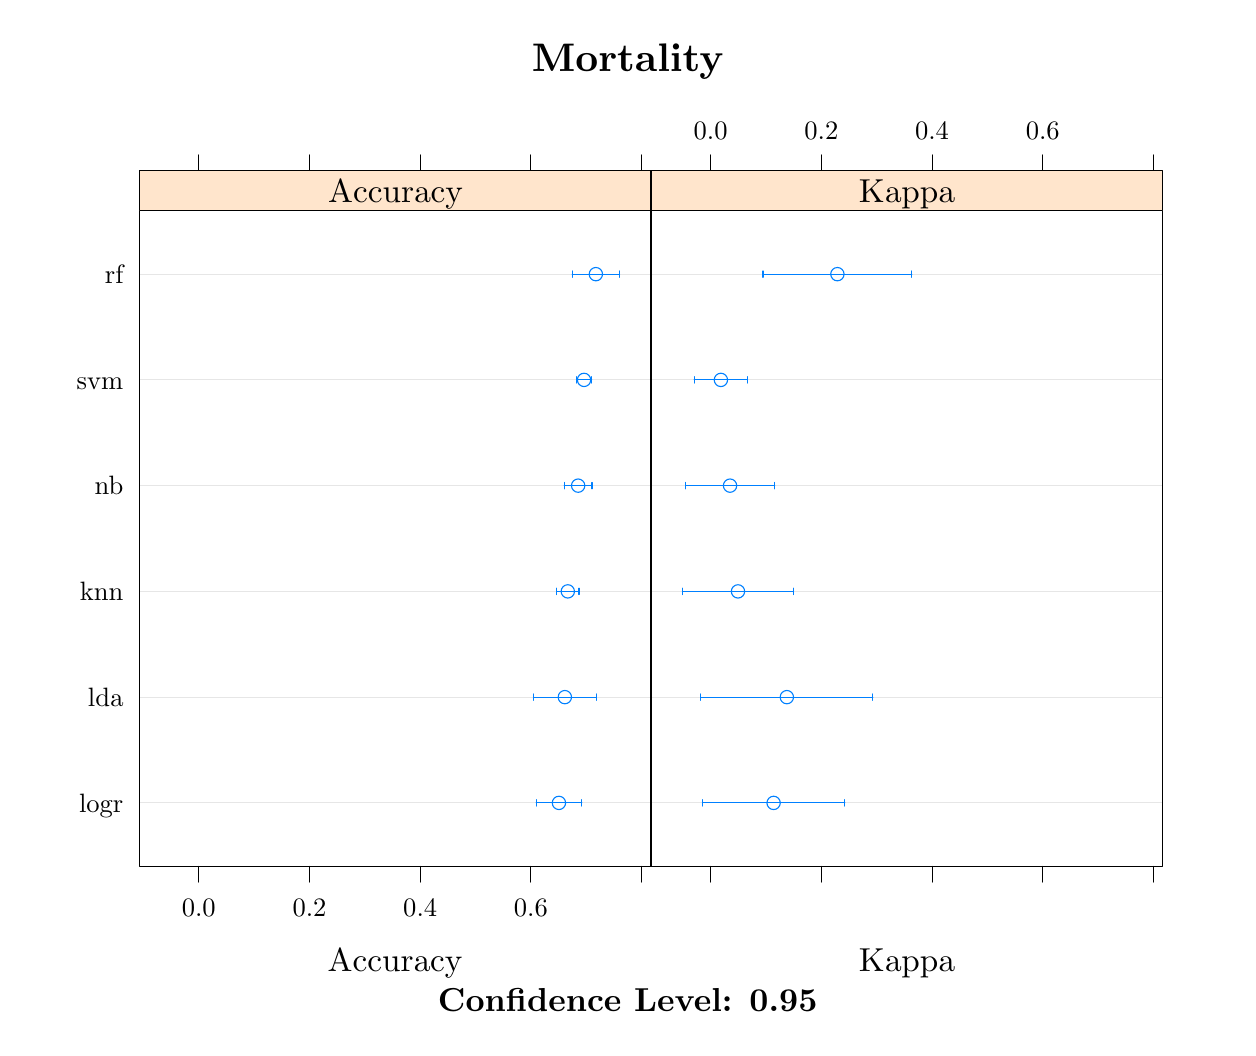
\begin{tikzpicture}[x=1pt,y=1pt]
\definecolor{fillColor}{RGB}{255,255,255}
\path[use as bounding box,fill=fillColor,fill opacity=0.00] (0,0) rectangle (433.62,361.35);
\begin{scope}
\path[clip] (  0.00,  0.00) rectangle (433.62,361.35);

\path[] (  0.00,  0.00) rectangle (433.62,361.35);
\definecolor{drawColor}{RGB}{0,0,0}

\node[text=drawColor,anchor=base,inner sep=0pt, outer sep=0pt, scale=  1.44] at (216.81,345.39) {\bfseries Mortality};
\end{scope}
\begin{scope}
\path[clip] (  0.00,  0.00) rectangle (433.62,361.35);
\definecolor{drawColor}{RGB}{0,0,0}

\node[text=drawColor,anchor=base,inner sep=0pt, outer sep=0pt, scale=  1.20] at (216.81,  6.02) {\bfseries Confidence Level: 0.95};
\end{scope}
\begin{scope}
\path[clip] (  0.00,  0.00) rectangle (433.62,361.35);
\definecolor{drawColor}{RGB}{0,0,0}

\node[text=drawColor,anchor=base,inner sep=0pt, outer sep=0pt, scale=  1.20] at (132.76, 20.33) {Accuracy};

\node[text=drawColor,anchor=base,inner sep=0pt, outer sep=0pt, scale=  1.20] at (317.71, 20.33) {Kappa};
\end{scope}
\begin{scope}
\path[clip] (  0.00,  0.00) rectangle (433.62,361.35);
\definecolor{drawColor}{RGB}{0,0,0}

\path[draw=drawColor,line width= 0.4pt,line join=round,line cap=round] ( 61.84,309.66) -- ( 61.84,315.35);

\path[draw=drawColor,line width= 0.4pt,line join=round,line cap=round] (101.84,309.66) -- (101.84,315.35);

\path[draw=drawColor,line width= 0.4pt,line join=round,line cap=round] (141.84,309.66) -- (141.84,315.35);

\path[draw=drawColor,line width= 0.4pt,line join=round,line cap=round] (181.84,309.66) -- (181.84,315.35);

\path[draw=drawColor,line width= 0.4pt,line join=round,line cap=round] (221.84,309.66) -- (221.84,315.35);
\end{scope}
\begin{scope}
\path[clip] (  0.00,  0.00) rectangle (433.62,361.35);
\definecolor{drawColor}{RGB}{0,0,0}

\node[text=drawColor,anchor=base east,inner sep=0pt, outer sep=0pt, scale=  0.96] at ( 34.58, 77.92) {logr};

\node[text=drawColor,anchor=base east,inner sep=0pt, outer sep=0pt, scale=  0.96] at ( 34.58,116.13) {lda};

\node[text=drawColor,anchor=base east,inner sep=0pt, outer sep=0pt, scale=  0.96] at ( 34.58,154.34) {knn};

\node[text=drawColor,anchor=base east,inner sep=0pt, outer sep=0pt, scale=  0.96] at ( 34.58,192.55) {nb};

\node[text=drawColor,anchor=base east,inner sep=0pt, outer sep=0pt, scale=  0.96] at ( 34.58,230.76) {svm};

\node[text=drawColor,anchor=base east,inner sep=0pt, outer sep=0pt, scale=  0.96] at ( 34.58,268.97) {rf};
\end{scope}
\begin{scope}
\path[clip] (  0.00,  0.00) rectangle (433.62,361.35);
\definecolor{drawColor}{RGB}{0,0,0}

\path[draw=drawColor,line width= 0.4pt,line join=round,line cap=round] ( 61.84, 58.30) -- ( 61.84, 52.61);

\path[draw=drawColor,line width= 0.4pt,line join=round,line cap=round] (101.84, 58.30) -- (101.84, 52.61);

\path[draw=drawColor,line width= 0.4pt,line join=round,line cap=round] (141.84, 58.30) -- (141.84, 52.61);

\path[draw=drawColor,line width= 0.4pt,line join=round,line cap=round] (181.84, 58.30) -- (181.84, 52.61);

\path[draw=drawColor,line width= 0.4pt,line join=round,line cap=round] (221.84, 58.30) -- (221.84, 52.61);

\node[text=drawColor,anchor=base,inner sep=0pt, outer sep=0pt, scale=  0.96] at ( 61.84, 40.30) {0.0};

\node[text=drawColor,anchor=base,inner sep=0pt, outer sep=0pt, scale=  0.96] at (101.84, 40.30) {0.2};

\node[text=drawColor,anchor=base,inner sep=0pt, outer sep=0pt, scale=  0.96] at (141.84, 40.30) {0.4};

\node[text=drawColor,anchor=base,inner sep=0pt, outer sep=0pt, scale=  0.96] at (181.84, 40.30) {0.6};
\end{scope}
\begin{scope}
\path[clip] ( 40.28, 58.30) rectangle (225.23,295.21);
\definecolor{drawColor}{RGB}{230,230,230}

\path[draw=drawColor,line width= 0.4pt,line join=round,line cap=round] ( 40.28, 81.22) -- (225.23, 81.22);

\path[draw=drawColor,line width= 0.4pt,line join=round,line cap=round] ( 40.28,119.44) -- (225.23,119.44);

\path[draw=drawColor,line width= 0.4pt,line join=round,line cap=round] ( 40.28,157.65) -- (225.23,157.65);

\path[draw=drawColor,line width= 0.4pt,line join=round,line cap=round] ( 40.28,195.86) -- (225.23,195.86);

\path[draw=drawColor,line width= 0.4pt,line join=round,line cap=round] ( 40.28,234.07) -- (225.23,234.07);

\path[draw=drawColor,line width= 0.4pt,line join=round,line cap=round] ( 40.28,272.28) -- (225.23,272.28);
\definecolor{drawColor}{RGB}{0,128,255}

\path[draw=drawColor,line width= 0.4pt,line join=round,line cap=round] (191.97, 81.22) circle (  2.41);

\path[draw=drawColor,line width= 0.4pt,line join=round,line cap=round] (194.11,119.44) circle (  2.41);

\path[draw=drawColor,line width= 0.4pt,line join=round,line cap=round] (195.17,157.65) circle (  2.41);

\path[draw=drawColor,line width= 0.4pt,line join=round,line cap=round] (198.91,195.86) circle (  2.41);

\path[draw=drawColor,line width= 0.4pt,line join=round,line cap=round] (201.04,234.07) circle (  2.41);

\path[draw=drawColor,line width= 0.4pt,line join=round,line cap=round] (205.31,272.28) circle (  2.41);

\path[draw=drawColor,line width= 0.4pt,line join=round,line cap=round] (183.73, 81.22) -- (200.22, 81.22);

\path[draw=drawColor,line width= 0.4pt,line join=round,line cap=round] (182.73,119.44) -- (205.48,119.44);

\path[draw=drawColor,line width= 0.4pt,line join=round,line cap=round] (191.12,157.65) -- (199.23,157.65);

\path[draw=drawColor,line width= 0.4pt,line join=round,line cap=round] (193.89,195.86) -- (203.93,195.86);

\path[draw=drawColor,line width= 0.4pt,line join=round,line cap=round] (198.27,234.07) -- (203.81,234.07);

\path[draw=drawColor,line width= 0.4pt,line join=round,line cap=round] (196.74,272.28) -- (213.88,272.28);

\path[draw=drawColor,line width= 0.4pt,line join=round,line cap=round] (183.73, 82.37) -- (183.73, 80.08);

\path[draw=drawColor,line width= 0.4pt,line join=round,line cap=round] (182.73,120.58) -- (182.73,118.29);

\path[draw=drawColor,line width= 0.4pt,line join=round,line cap=round] (191.12,158.79) -- (191.12,156.50);

\path[draw=drawColor,line width= 0.4pt,line join=round,line cap=round] (193.89,197.00) -- (193.89,194.71);

\path[draw=drawColor,line width= 0.4pt,line join=round,line cap=round] (198.27,235.22) -- (198.27,232.92);

\path[draw=drawColor,line width= 0.4pt,line join=round,line cap=round] (196.74,273.43) -- (196.74,271.13);

\path[draw=drawColor,line width= 0.4pt,line join=round,line cap=round] (200.22, 82.37) -- (200.22, 80.08);

\path[draw=drawColor,line width= 0.4pt,line join=round,line cap=round] (205.48,120.58) -- (205.48,118.29);

\path[draw=drawColor,line width= 0.4pt,line join=round,line cap=round] (199.23,158.79) -- (199.23,156.50);

\path[draw=drawColor,line width= 0.4pt,line join=round,line cap=round] (203.93,197.00) -- (203.93,194.71);

\path[draw=drawColor,line width= 0.4pt,line join=round,line cap=round] (203.81,235.22) -- (203.81,232.92);

\path[draw=drawColor,line width= 0.4pt,line join=round,line cap=round] (213.88,273.43) -- (213.88,271.13);
\end{scope}
\begin{scope}
\path[clip] (  0.00,  0.00) rectangle (433.62,361.35);
\definecolor{drawColor}{RGB}{0,0,0}

\path[draw=drawColor,line width= 0.4pt,line join=round,line cap=round] ( 40.28, 58.30) rectangle (225.23,295.21);
\end{scope}
\begin{scope}
\path[clip] ( 40.28,295.21) rectangle (225.23,309.66);
\definecolor{drawColor}{RGB}{255,229,204}
\definecolor{fillColor}{RGB}{255,229,204}

\path[draw=drawColor,line width= 0.4pt,line join=round,line cap=round,fill=fillColor] ( 40.28,295.21) rectangle (225.23,309.66);
\definecolor{drawColor}{RGB}{0,0,0}

\node[text=drawColor,anchor=base west,inner sep=0pt, outer sep=0pt, scale=  1.20] at (108.58,298.30) {Accuracy};
\end{scope}
\begin{scope}
\path[clip] (  0.00,  0.00) rectangle (433.62,361.35);
\definecolor{drawColor}{RGB}{0,0,0}

\path[draw=drawColor,line width= 0.4pt,line join=round,line cap=round] ( 40.28,295.21) rectangle (225.23,309.66);
\end{scope}
\begin{scope}
\path[clip] (  0.00,  0.00) rectangle (433.62,361.35);
\definecolor{drawColor}{RGB}{0,0,0}

\path[draw=drawColor,line width= 0.4pt,line join=round,line cap=round] (246.80,309.66) -- (246.80,315.35);

\path[draw=drawColor,line width= 0.4pt,line join=round,line cap=round] (286.80,309.66) -- (286.80,315.35);

\path[draw=drawColor,line width= 0.4pt,line join=round,line cap=round] (326.80,309.66) -- (326.80,315.35);

\path[draw=drawColor,line width= 0.4pt,line join=round,line cap=round] (366.80,309.66) -- (366.80,315.35);

\path[draw=drawColor,line width= 0.4pt,line join=round,line cap=round] (406.80,309.66) -- (406.80,315.35);

\node[text=drawColor,anchor=base,inner sep=0pt, outer sep=0pt, scale=  0.96] at (246.80,321.04) {0.0};

\node[text=drawColor,anchor=base,inner sep=0pt, outer sep=0pt, scale=  0.96] at (286.80,321.04) {0.2};

\node[text=drawColor,anchor=base,inner sep=0pt, outer sep=0pt, scale=  0.96] at (326.80,321.04) {0.4};

\node[text=drawColor,anchor=base,inner sep=0pt, outer sep=0pt, scale=  0.96] at (366.80,321.04) {0.6};
\end{scope}
\begin{scope}
\path[clip] (  0.00,  0.00) rectangle (433.62,361.35);
\definecolor{drawColor}{RGB}{0,0,0}

\path[draw=drawColor,line width= 0.4pt,line join=round,line cap=round] (246.80, 58.30) -- (246.80, 52.61);

\path[draw=drawColor,line width= 0.4pt,line join=round,line cap=round] (286.80, 58.30) -- (286.80, 52.61);

\path[draw=drawColor,line width= 0.4pt,line join=round,line cap=round] (326.80, 58.30) -- (326.80, 52.61);

\path[draw=drawColor,line width= 0.4pt,line join=round,line cap=round] (366.80, 58.30) -- (366.80, 52.61);

\path[draw=drawColor,line width= 0.4pt,line join=round,line cap=round] (406.80, 58.30) -- (406.80, 52.61);
\end{scope}
\begin{scope}
\path[clip] (225.23, 58.30) rectangle (410.19,295.21);
\definecolor{drawColor}{RGB}{230,230,230}

\path[draw=drawColor,line width= 0.4pt,line join=round,line cap=round] (225.23, 81.22) -- (410.19, 81.22);

\path[draw=drawColor,line width= 0.4pt,line join=round,line cap=round] (225.23,119.44) -- (410.19,119.44);

\path[draw=drawColor,line width= 0.4pt,line join=round,line cap=round] (225.23,157.65) -- (410.19,157.65);

\path[draw=drawColor,line width= 0.4pt,line join=round,line cap=round] (225.23,195.86) -- (410.19,195.86);

\path[draw=drawColor,line width= 0.4pt,line join=round,line cap=round] (225.23,234.07) -- (410.19,234.07);

\path[draw=drawColor,line width= 0.4pt,line join=round,line cap=round] (225.23,272.28) -- (410.19,272.28);
\definecolor{drawColor}{RGB}{0,128,255}

\path[draw=drawColor,line width= 0.4pt,line join=round,line cap=round] (269.54, 81.22) circle (  2.41);

\path[draw=drawColor,line width= 0.4pt,line join=round,line cap=round] (274.33,119.44) circle (  2.41);

\path[draw=drawColor,line width= 0.4pt,line join=round,line cap=round] (256.67,157.65) circle (  2.41);

\path[draw=drawColor,line width= 0.4pt,line join=round,line cap=round] (253.80,195.86) circle (  2.41);

\path[draw=drawColor,line width= 0.4pt,line join=round,line cap=round] (250.49,234.07) circle (  2.41);

\path[draw=drawColor,line width= 0.4pt,line join=round,line cap=round] (292.59,272.28) circle (  2.41);

\path[draw=drawColor,line width= 0.4pt,line join=round,line cap=round] (243.81, 81.22) -- (295.28, 81.22);

\path[draw=drawColor,line width= 0.4pt,line join=round,line cap=round] (243.25,119.44) -- (305.40,119.44);

\path[draw=drawColor,line width= 0.4pt,line join=round,line cap=round] (236.59,157.65) -- (276.74,157.65);

\path[draw=drawColor,line width= 0.4pt,line join=round,line cap=round] (237.66,195.86) -- (269.94,195.86);

\path[draw=drawColor,line width= 0.4pt,line join=round,line cap=round] (240.87,234.07) -- (260.12,234.07);

\path[draw=drawColor,line width= 0.4pt,line join=round,line cap=round] (265.69,272.28) -- (319.50,272.28);

\path[draw=drawColor,line width= 0.4pt,line join=round,line cap=round] (243.81, 82.37) -- (243.81, 80.08);

\path[draw=drawColor,line width= 0.4pt,line join=round,line cap=round] (243.25,120.58) -- (243.25,118.29);

\path[draw=drawColor,line width= 0.4pt,line join=round,line cap=round] (236.59,158.79) -- (236.59,156.50);

\path[draw=drawColor,line width= 0.4pt,line join=round,line cap=round] (237.66,197.00) -- (237.66,194.71);

\path[draw=drawColor,line width= 0.4pt,line join=round,line cap=round] (240.87,235.22) -- (240.87,232.92);

\path[draw=drawColor,line width= 0.4pt,line join=round,line cap=round] (265.69,273.43) -- (265.69,271.13);

\path[draw=drawColor,line width= 0.4pt,line join=round,line cap=round] (295.28, 82.37) -- (295.28, 80.08);

\path[draw=drawColor,line width= 0.4pt,line join=round,line cap=round] (305.40,120.58) -- (305.40,118.29);

\path[draw=drawColor,line width= 0.4pt,line join=round,line cap=round] (276.74,158.79) -- (276.74,156.50);

\path[draw=drawColor,line width= 0.4pt,line join=round,line cap=round] (269.94,197.00) -- (269.94,194.71);

\path[draw=drawColor,line width= 0.4pt,line join=round,line cap=round] (260.12,235.22) -- (260.12,232.92);

\path[draw=drawColor,line width= 0.4pt,line join=round,line cap=round] (319.50,273.43) -- (319.50,271.13);
\end{scope}
\begin{scope}
\path[clip] (  0.00,  0.00) rectangle (433.62,361.35);
\definecolor{drawColor}{RGB}{0,0,0}

\path[draw=drawColor,line width= 0.4pt,line join=round,line cap=round] (225.23, 58.30) rectangle (410.19,295.21);
\end{scope}
\begin{scope}
\path[clip] (225.23,295.21) rectangle (410.19,309.66);
\definecolor{drawColor}{RGB}{255,229,204}
\definecolor{fillColor}{RGB}{255,229,204}

\path[draw=drawColor,line width= 0.4pt,line join=round,line cap=round,fill=fillColor] (225.23,295.21) rectangle (410.19,309.66);
\definecolor{drawColor}{RGB}{0,0,0}

\node[text=drawColor,anchor=base west,inner sep=0pt, outer sep=0pt, scale=  1.20] at (300.39,298.30) {Kappa};
\end{scope}
\begin{scope}
\path[clip] (  0.00,  0.00) rectangle (433.62,361.35);
\definecolor{drawColor}{RGB}{0,0,0}

\path[draw=drawColor,line width= 0.4pt,line join=round,line cap=round] (225.23,295.21) rectangle (410.19,309.66);
\end{scope}
\end{tikzpicture}
